%!TEX root = THinstituteReport_1.tex
%\newpage
%%%%%%%%%%%%%%%%%%%%%%%%%%%%%%%%%%%%%%%%%%
\section{Background subtraction methods}
\label{app:background}
%%%%%%%%%%%%%%%%%%%%%%%%%%%%%%%%%%%%%%%%%%

This sections provides some details about methods for background subtraction. We were mainly focussing on applications using area-based subtraction, constituent subtraction (CS) \cite{Berta:2014eza} and Soft Killer (SK) \cite{Cacciari:2014gra}. The subtraction methods are evaluated by embedding jets generated with PYTHIA into a background resembling the properties of the underlying event observed at the LHC. The underlying event is generated assuming independent particle production according to a thermal Boltzmann distribution \cite{deBarros:2012ws}. Massless particles are generated randomly at central rapidities $|\eta|<3$. A Boltzmann distribution, with $\langle \pT \rangle$ = 1.2 GeV is used. This is equivalent to an average momentum density of $\langle \rho \rangle =250$ GeV and a total multiplicity of $\sim 7000$ particles, which corresponds roughly to the most central events in the CMS detector. \autoref{fig:ResponseMethods} shows the jet response for the transverse momentum (left) and mass (right) for the two background subtraction methods mentioned before. For both methods a free tunable parameter exists and we show the jet response for two different choices. The constituent subtraction is not very sensitive to the parameter $\alpha$ that regulates the $p_{\mathrm{T}}$ weighting of the distance parameter used in the algorithm. The response of Soft Killer is very sensitive to the width ($w$) used. By default the values is 0.4 but we observe that in the heavy ion environment a better performance is achieved using a smaller value since otherwise the algorithm subtracts part of the true jet signal.


%%%%%%%%%%%%%%%%%%%%%%%%%%%%%%%%%%%%%
\begin{figure}[h!]
\centering
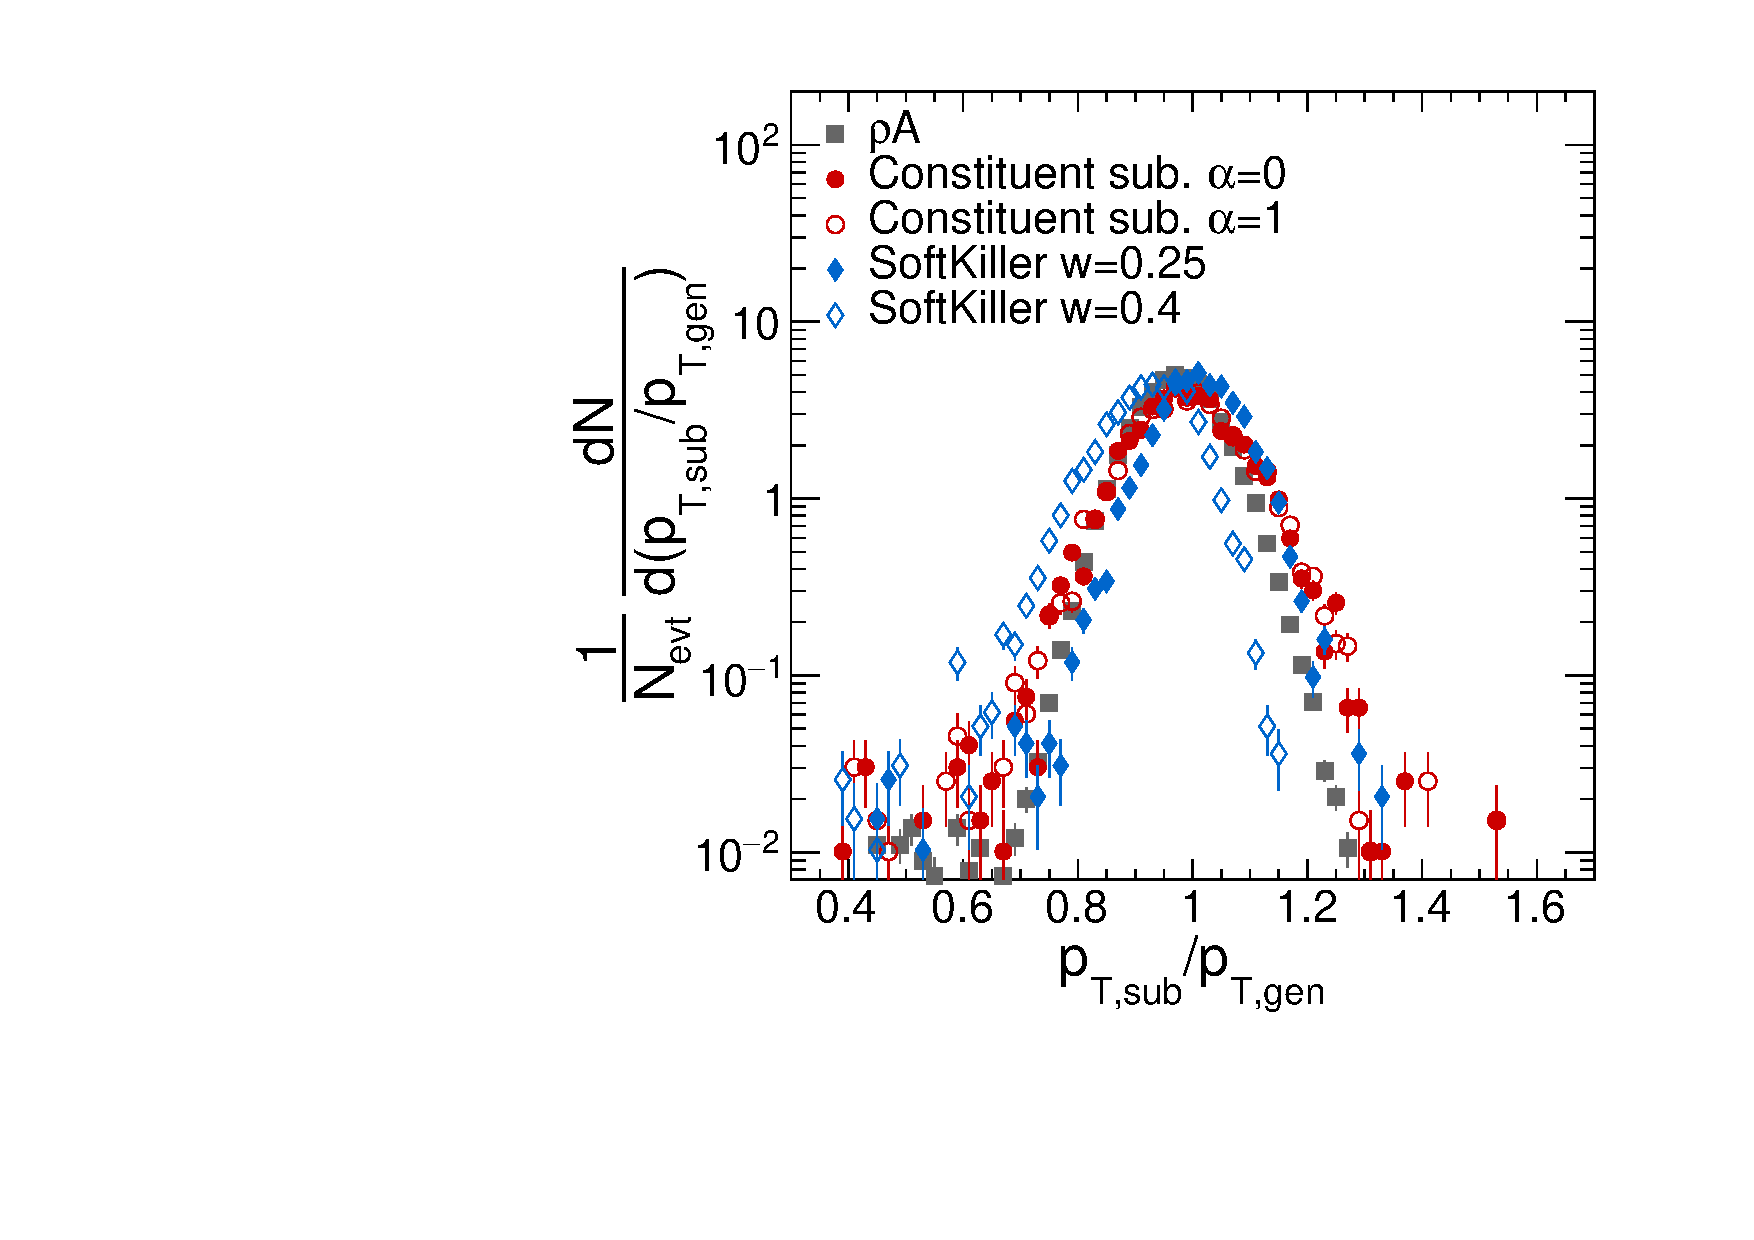
\includegraphics[width=0.5\textwidth]{figures/bkgMethods/JetPtResponseMethods.pdf}%
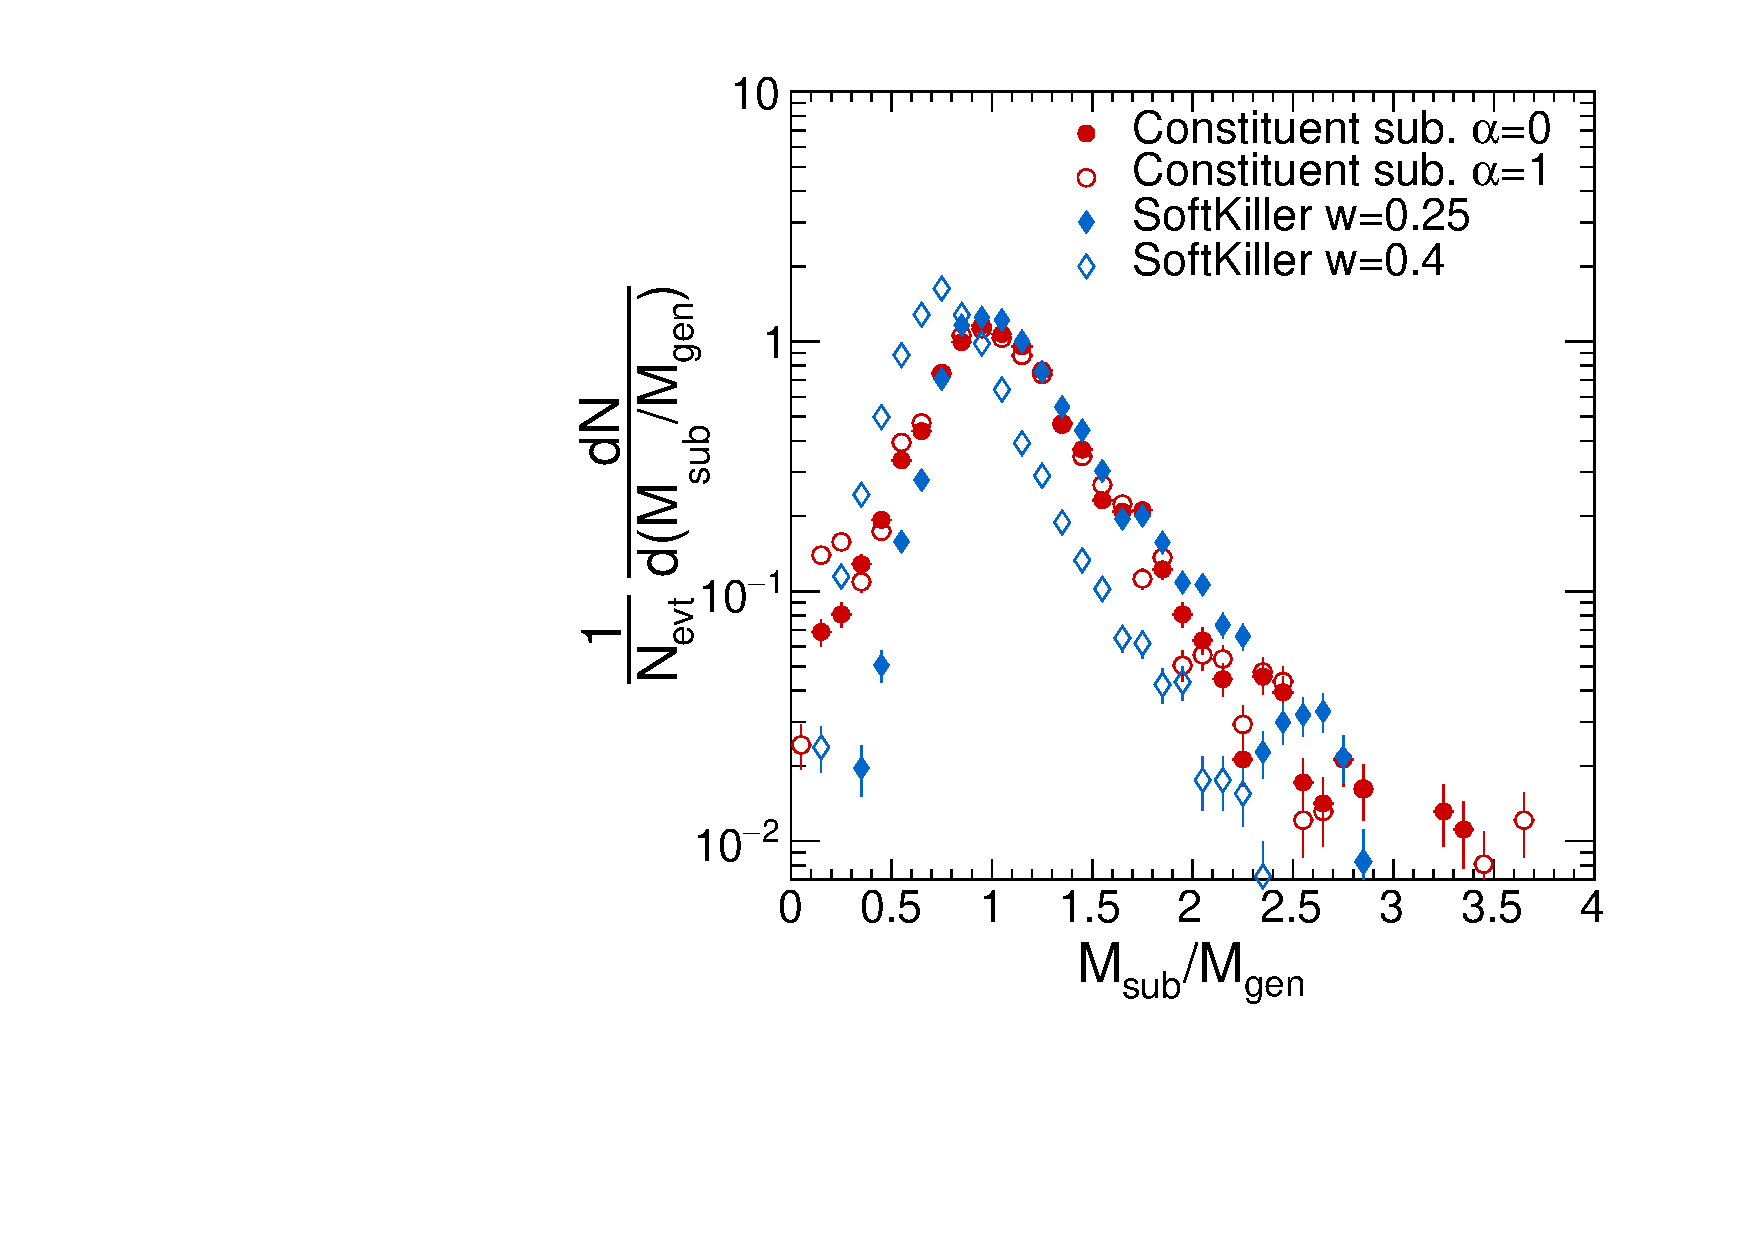
\includegraphics[width=0.5\textwidth]{figures/bkgMethods/JetMassResponseMethods.pdf}%
\caption{Jet energy (left) and mass response (right) for various jet subtraction techniques. PYTHIA jets are embedded into a thermal background corresponding to the characteriques observed in central PbPb collisions at the LHC.}
\label{fig:ResponseMethods}
\end{figure}
%%%%%%%%%%%%%%%%%%%%%%%%%%%%%%%%%%%%%
